\documentclass[]{article}
\usepackage{graphicx}
\graphicspath{{./images/}}

%opening
\title{Edison to Android Bluetooth Communications}
\author{Junchao Zhou \and Matthew Swartouwt \and James Zhang}

\begin{document}

\maketitle

\section{Homework 1}
Homoework 1 was very simple. We modified the Grove Indoor Environment Demo to also write to the SD card. First, we removed all of the WiFi components of the demo because they were not necessary for this and would cause the program to stall when it couldn't connect to a WiFi network. Then, we added a small section of code to the setup loop to create the homework1.txt file on the SD card if it doesn't exist. Next, we modified the printSettings method and every time that a sensor measurement is written to the screen we also wrote it to the SD card. Finally, we added a call to printSettings in the main loop so that each time the loop executes it prints the sensor values to the terminal and also writes them to the SD card. A video can be found in the videos/ directory showing homework1 in action.
 
\section{Python Part}
Modifying the SPP-loopback.py method was also very simple. We first used the mraa package to associate pins with their sensor. Then, in the main loop, we added logic to start the feedback loop. The loop receives a data value from the bluetooth app. If that message is not "start" then the loop waits for another message. If that message is "start" then the loop will read each sensor value and then send it over Bluetooth to the client. It will also print out the measured sensor value in the local serial terminal. These modifications were very simple and minimal. 

\section{Android Part}
Generally speaking, we just modified the official BluetoothChat example to get our own Android Bluetooth client for Edison board. 

The idea of ActionBar used in BluetoothChat example is very useful. I first set the menu to “android\_client\_for\_edison.xml” which includes three buttons, “Connect a device – Secure”, “Connect a device – Insecure”, “Make Discoverable”. For each menu item, set android:showAsAction entry to let each item shown on the bar or not.
 
Then in MainActivity, inplement the onOptionsItemSelected(MenuItem item) method. When an item is clicked, it will start a DeviceListActivity either secure or insecure to show the paired devices or scan for new devices.  

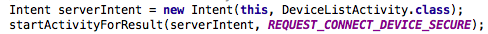
\includegraphics[keepaspectratio, width=\textwidth]{codeSnippet1}

Then we can click the device which we want to connect and the DeviceListActivity will return the device address to the MainActivity which called the startActivityForResult(…) method using the intent.putExtra shown in the figure.

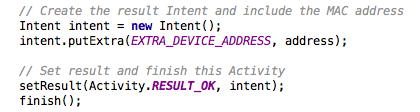
\includegraphics[keepaspectratio, width=\textwidth]{codeSnippet2}

Then in the MainActivity, we can implement onActivityResult() method to deal with the result and call connectDevice() method to connect the Device which we selected. The connectDevice() method will call mChatService.connect(device, secure) to do the Bluetooth client job.


The BluetoothChatService is a user-defined class which implements Bluetooth communication. In this class, three important user-defined classes are AcceptThread, ConnectThread and ConnectedThread. It is necessary to run server accept(), client connect(), and read/write data in separate thread so that they will not block UI thread. 

Finally, we need a handler to transfer the received message to the UI. The handler mHandler is also an argument passed to mChatService object when we first initiate it by using “new BluetoothChatService(this, mHandler)”. In BluetoothChatService class, it will deliver a message indicating what the communication state is such as STATE\_CONNECTED or STATE\_NONE, and also a message indicating whether we are writing or reading data to the remote device. The mHandler will also set the Application’s subtitle indicating what the connection state is such as “connecting”, “connected” or “not connected”.  Also, when we receive MESSAGE\_READ, we need to save the incoming data stream to a CSV file. 

A video can be found in the videos/ directory of our project that shows the app running.

Additionally, see below for a few screenshots of the Android client being used to connect to a device and send messages over Bluetooth.

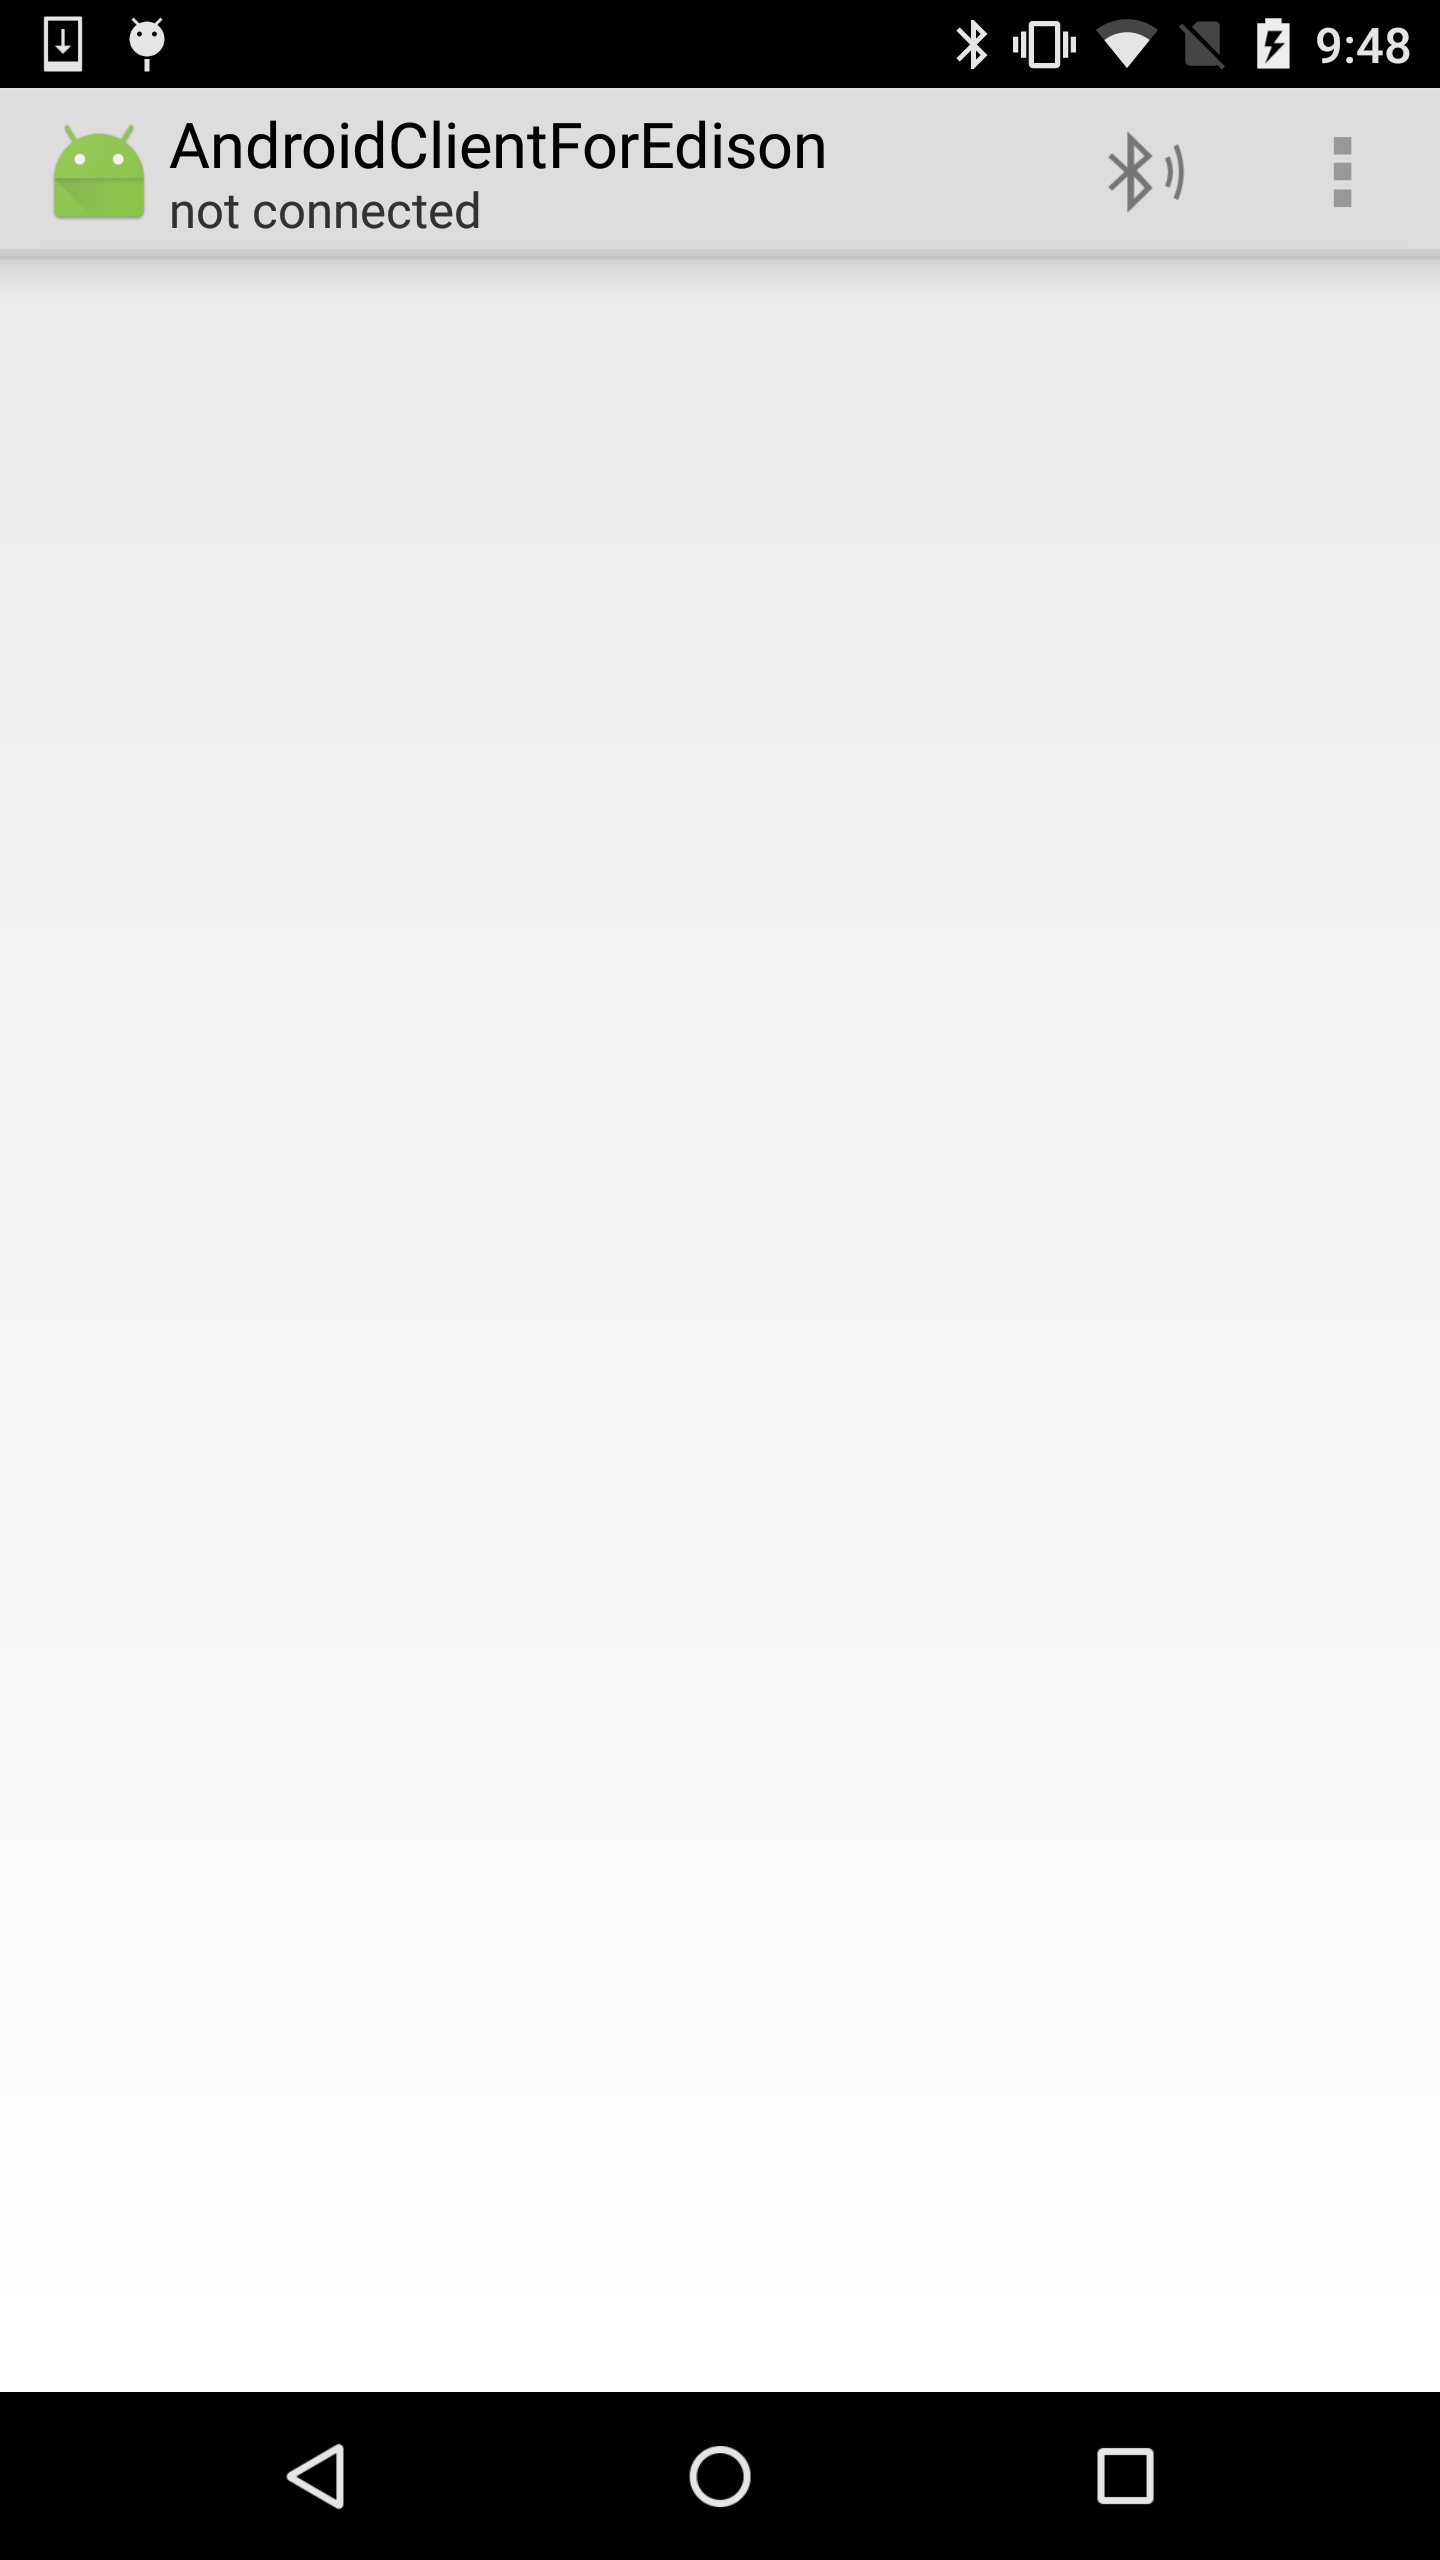
\includegraphics[keepaspectratio, width=\textwidth]{photo1}
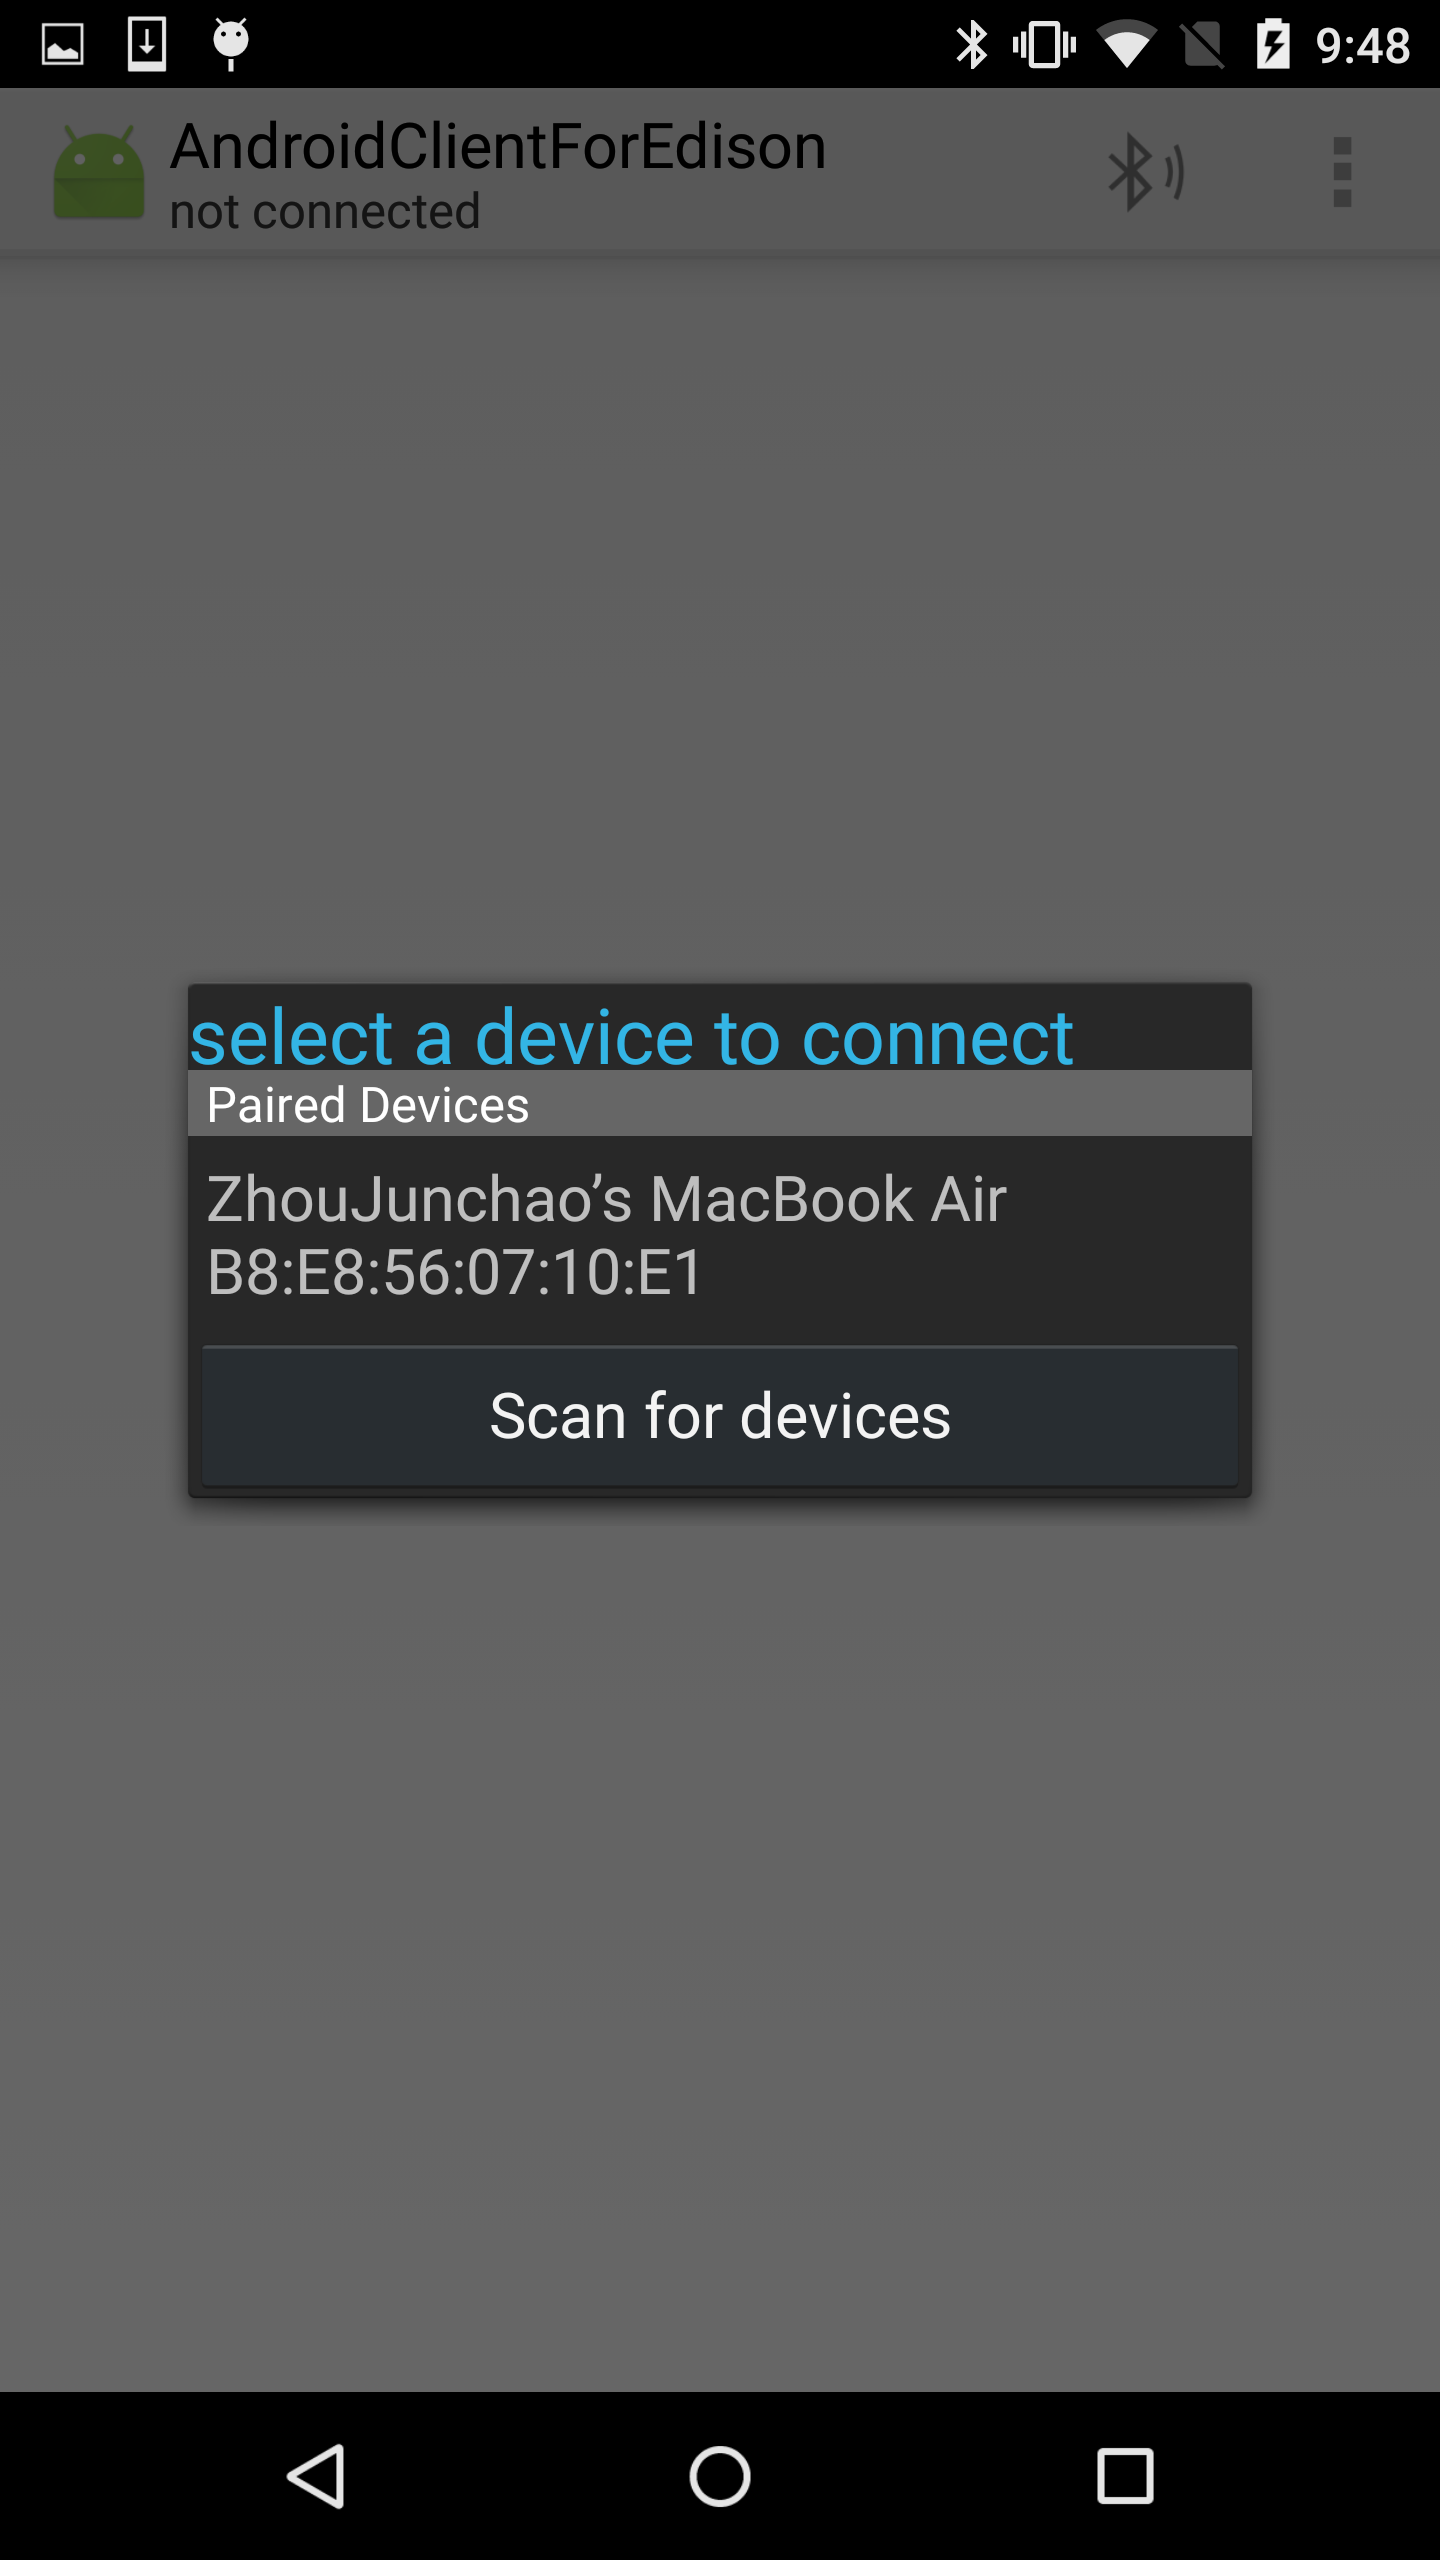
\includegraphics[keepaspectratio, width=\textwidth]{photo2}
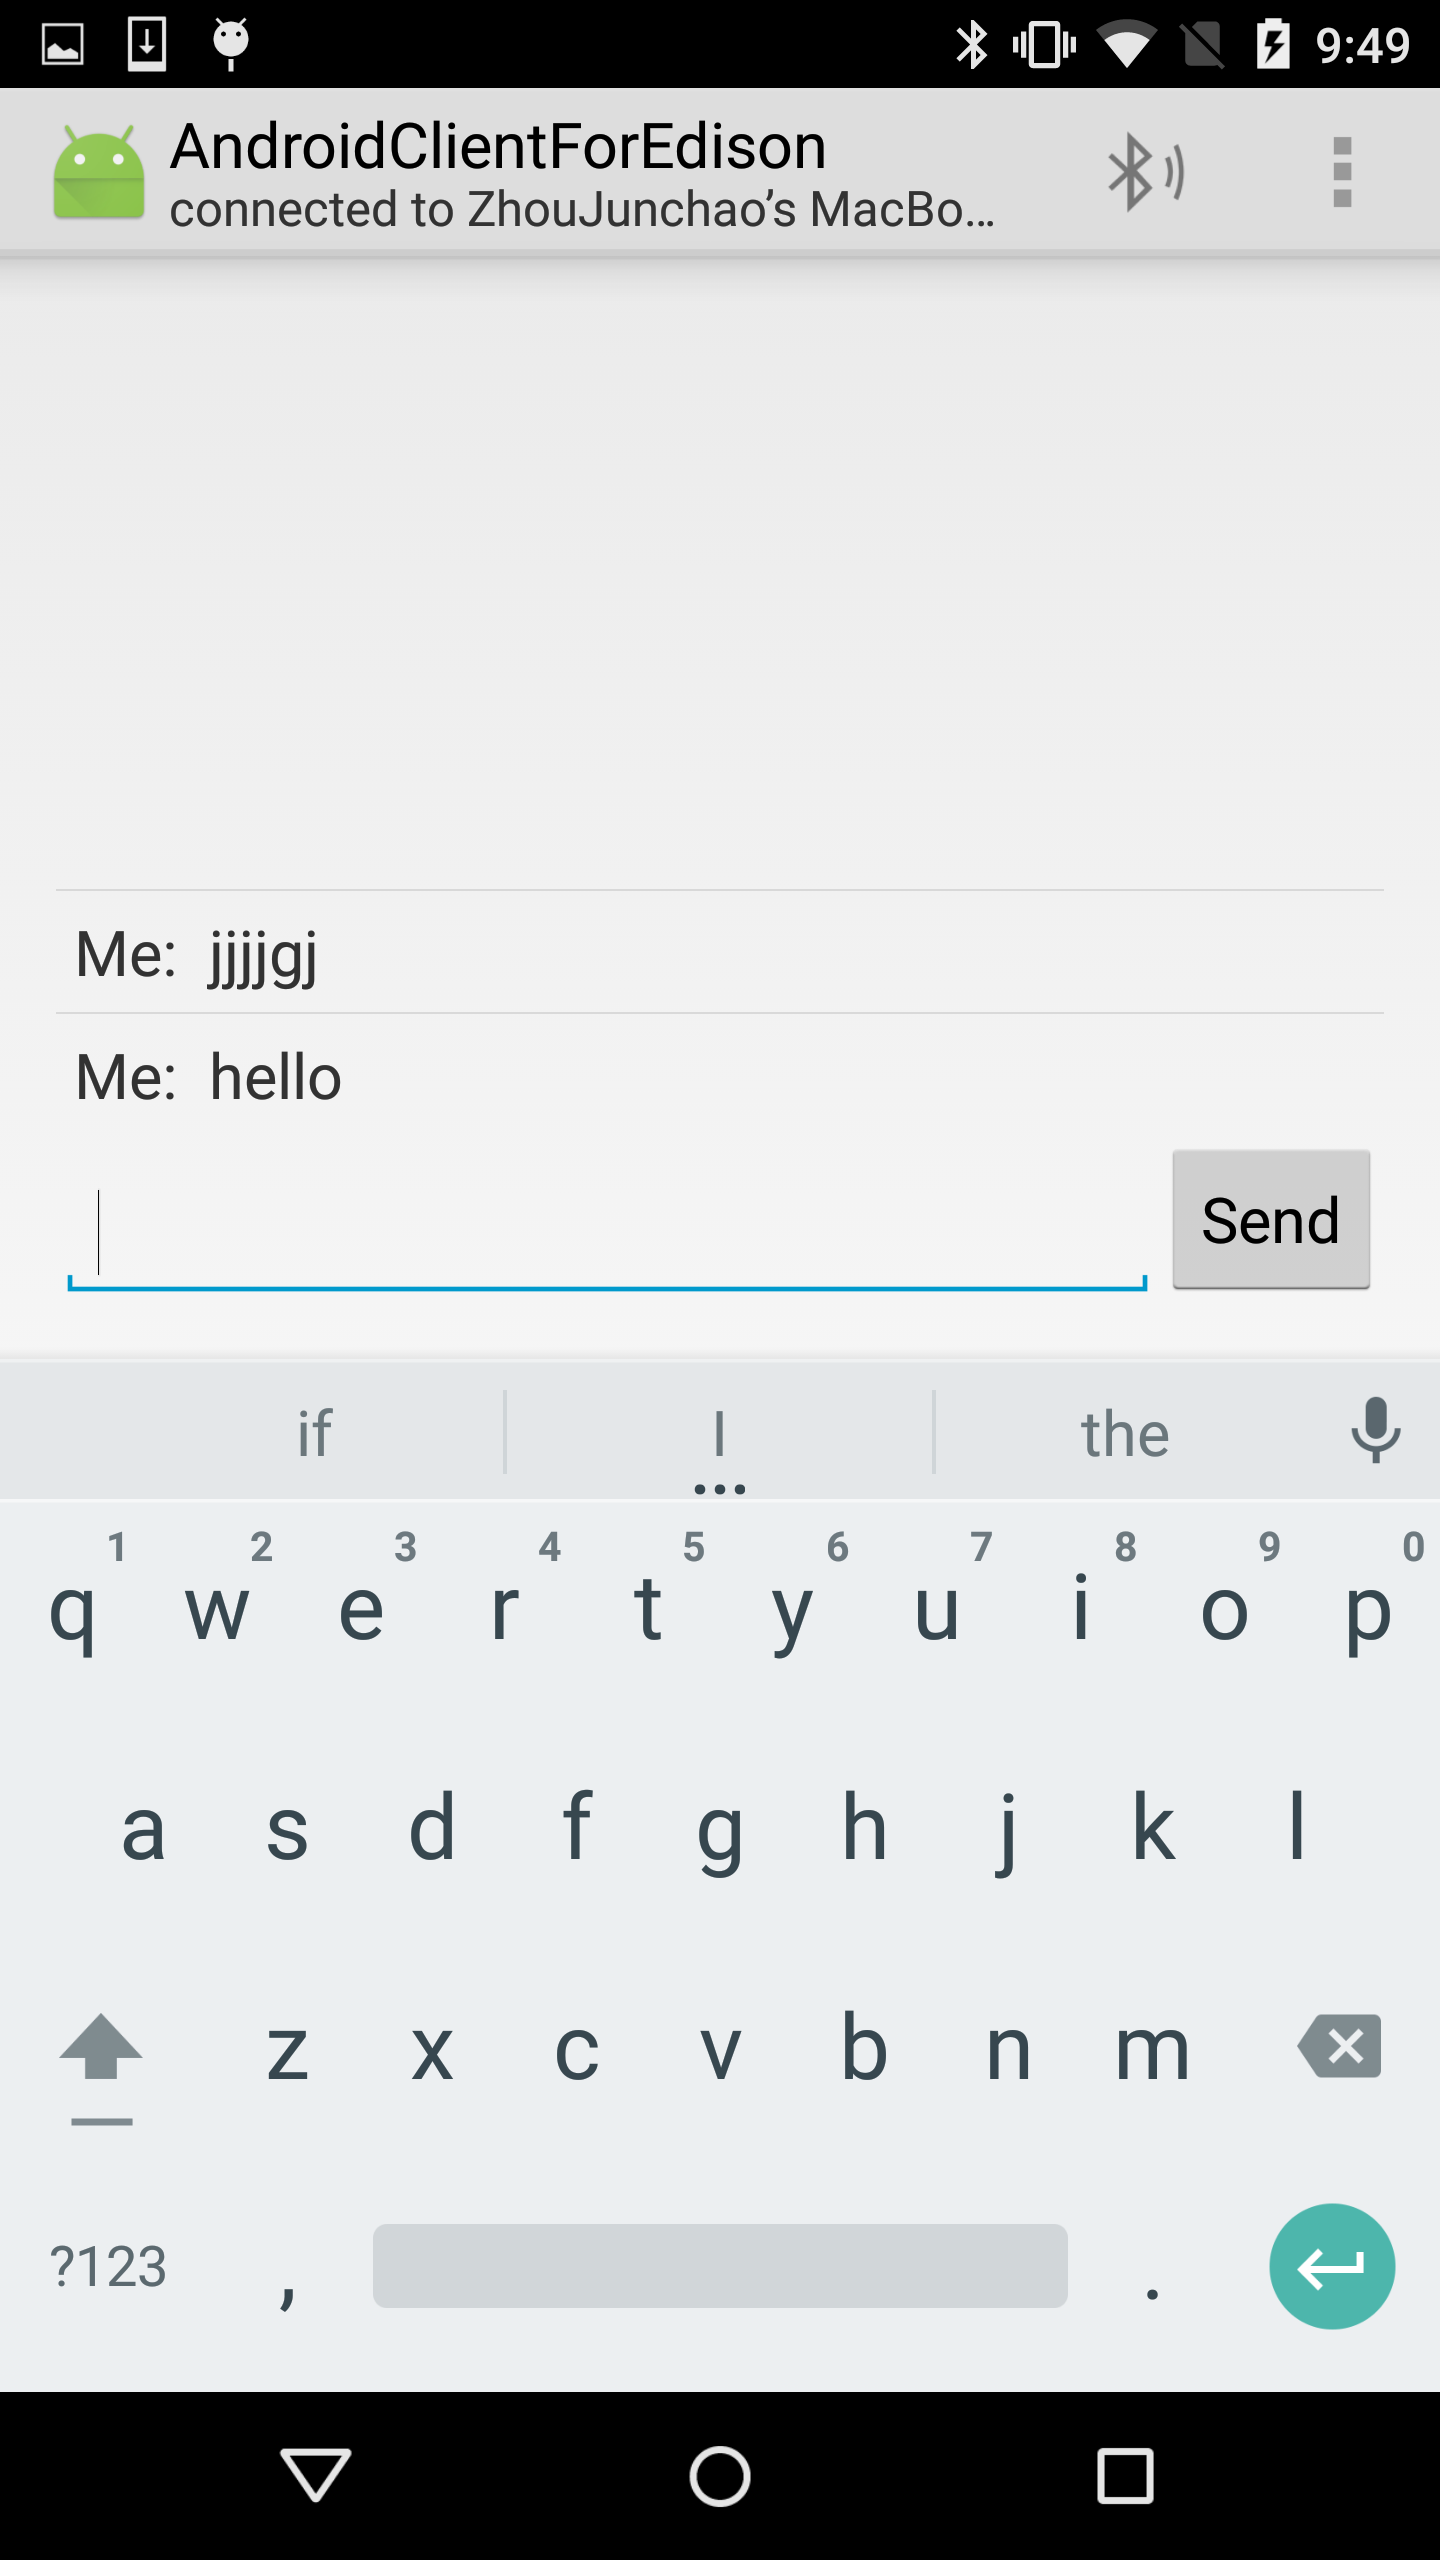
\includegraphics[keepaspectratio, width=\textwidth]{photo3}

\section{Contributions}
Junchao - Completed Homework 3 and assisted with Homework 2 debugging
Matt - Completed Homework 1 and all Python programming for Homework 2
James - Assisted with Homework 1 and 2 testing and debugging

\end{document}